%%%%%%%%%%%%%%%%%%%%%%%%%%%%%%%%%%%%%%%%%%%%%%%%%%%%%%%%%%%%%%%%%%%%%%%%%%%%%%%
% SPARTAN-16 — CMPE-220 CPU Design report (single file, pdfLaTeX / Overleaf)
%
% Repository: https://github.com/Ganeshmohank/220-A
% Format:     double-spaced body, 1in margins, page numbers after title,
%             dedicated pages for GitHub, build/run, contributions (Canvas).
%
% EDIT before final PDF: \SubmissionDate, \FibonacciVideoURL, and contribution
% bullets if your instructor expects a different team split.
%%%%%%%%%%%%%%%%%%%%%%%%%%%%%%%%%%%%%%%%%%%%%%%%%%%%%%%%%%%%%%%%%%%%%%%%%%%%%%%

\documentclass[12pt]{article}

\usepackage[margin=1in]{geometry}
\usepackage{setspace}
\usepackage{graphicx}
\usepackage{hyperref}
\usepackage{booktabs}
\usepackage{array}
\usepackage{parskip}
\usepackage{listings}
\usepackage{xcolor}
\usepackage{tikz}
\usetikzlibrary{arrows.meta,positioning}

\hypersetup{colorlinks=true,linkcolor=black,urlcolor=blue,citecolor=black}

\lstdefinestyle{shell}{
  basicstyle=\ttfamily\small,
  breaklines=true,
  frame=single,
  backgroundcolor=\color{gray!8},
  columns=fullflexible
}
\lstset{style=shell}

\newcommand{\UniversityLine}{San Jos\'{e} State University}
\newcommand{\CourseNumberName}{SP26: CMPE-220 Sec 01 --- System Software}
\newcommand{\ProjectTitle}{SPARTAN-16 --- Software CPU Emulator \& Assembler}
\newcommand{\AssignmentTitle}{CPU Design}
\newcommand{\SubmissionDate}{May 9, 2026}
\newcommand{\GitHubURL}{https://github.com/Ganeshmohank/220-A}
\newcommand{\GitHubCloneURL}{https://github.com/Ganeshmohank/220-A.git}
\newcommand{\FibonacciVideoURL}{https://youtu.be/REPLACE\_WITH\_YOUR\_VIDEO\_ID}
\newcommand{\TeamMemberOne}{Yaswanth Venkata Satya Naga Sa Dokala}
\newcommand{\TeamMemberTwo}{Siddharth Pawar Jetling}
\newcommand{\TeamMemberThree}{Ganesh Nagavenkatasai Mohan Kancherla}
\newcommand{\TeamMemberFour}{Sriyavarma Saripella}

\begin{document}

\begin{titlepage}
  \centering
  \vspace*{0.95in}
  {\large \UniversityLine\par}
  \vspace{0.35in}
  {\Large\bfseries \CourseNumberName\par}
  \vspace{0.45in}
  {\LARGE\bfseries \ProjectTitle\par}
  \vspace{0.22in}
  {\large \AssignmentTitle\par}
  \vspace{0.28in}
  {\large \SubmissionDate\par}
  \vfill
  \begin{flushleft}
    \large\textbf{Team members}\\[0.4em]
    \begin{itemize}\setlength\itemsep{0.18em}
      \item \TeamMemberOne
      \item \TeamMemberTwo
      \item \TeamMemberThree
      \item \TeamMemberFour
    \end{itemize}
  \end{flushleft}
  \vspace{0.5in}
\end{titlepage}
\thispagestyle{empty}
\clearpage

\setcounter{page}{1}
\pagestyle{plain}
\doublespacing

\section*{GitHub repository}
\addcontentsline{toc}{section}{GitHub repository}
\noindent\textbf{Repository URL (code, \texttt{docs/}, programs, build scripts):}\\[0.55em]
{\large\url{\GitHubURL}}

\noindent Canonical clone command:
\begin{center}
  \ttfamily git clone \url{\GitHubCloneURL}
\end{center}

\noindent The Fibonacci demo video required by the course must be reachable from this repository (for example linked in \texttt{README.md} or stored under \texttt{docs/}).
\vfill
\clearpage

\section*{Download, compile, and run}
\addcontentsline{toc}{section}{Download, compile, and run}
\noindent These steps mirror \texttt{README.md} on \texttt{main} so a grader can download and run on the first attempt.

\textbf{Prerequisites:} \texttt{make} and \texttt{g++} with C++17 (macOS or Linux; on Windows use WSL2 Ubuntu and the same commands).

\begin{enumerate}
  \item \textbf{Clone} (or download ZIP and extract):
  \begin{center}
    \ttfamily git clone \url{\GitHubCloneURL}
  \end{center}
  \item \textbf{Enter} the repository folder (default name \texttt{220-A/}). If your folder name contains spaces, quote the path when using \texttt{cd}.
\end{enumerate}

\subsection*{Build and quick demo}
\begin{lstlisting}
cd 220-A
chmod +x demo.sh
make
./demo.sh
\end{lstlisting}

\noindent\texttt{./demo.sh} defaults to Hello World; you can pass \texttt{fibonacci} or \texttt{timer}:
\begin{lstlisting}
./demo.sh fibonacci
./demo.sh timer
\end{lstlisting}

\subsection*{Run assembled programs directly (after \texttt{make})}
\begin{lstlisting}
./cpu exec programs/hello.asm
./cpu exec programs/fibonacci.asm
./cpu exec programs/timer.asm
\end{lstlisting}

\subsection*{Trace, dump, assemble-only, and Makefile shortcuts}
\begin{lstlisting}
./cpu exec programs/hello.asm --trace
./cpu exec programs/hello.asm --dump
./cpu assemble programs/fibonacci.asm -o fibonacci.bin
./cpu run fibonacci.bin
make clean
make hello
make fibonacci
make timer
make trace-fibonacci
make dump-hello
\end{lstlisting}
\vfill
\clearpage

\section*{Team member contributions}
\addcontentsline{toc}{section}{Team member contributions}
\noindent All four members shared responsibility for this PDF (\textbf{approximately 25\% each}): we held a joint planning pass against the Canvas instructions, split primary drafting by section, then \textbf{cross-reviewed} every page so wording, commands, and rubric coverage are consistent.

\begin{table}[h!]
  \centering
  \renewcommand{\arraystretch}{1.22}
  \begin{tabular}{>{\raggedright\arraybackslash}p{2.35in} >{\raggedright\arraybackslash}p{4.1in}}
    \toprule
    \textbf{Team member} & \textbf{Contribution summary (course report)} \\
    \midrule
    \TeamMemberOne &
    \begin{minipage}[t]{\linewidth}\raggedright
      \begin{itemize}\setlength\itemsep{0.05em}
        \item Primary draft of the \textbf{title page} and \textbf{GitHub repository} pages; standardized course header and submission metadata.
        \item Co-edited \textbf{ISA} subsections (instruction format, opcodes, flags) and participated in full-document proofreading pass.
      \end{itemize}
    \end{minipage} \\
    \midrule
    \TeamMemberTwo &
    \begin{minipage}[t]{\linewidth}\raggedright
      \begin{itemize}\setlength\itemsep{0.05em}
        \item Primary draft of \textbf{Download, compile, and run} from the live \texttt{README.md}; verified \texttt{make}, \texttt{demo.sh}, and \texttt{./cpu exec} commands on a clean clone.
        \item Co-edited \textbf{Emulator} and \textbf{Assembler} subsections to match repository filenames and behavior.
      \end{itemize}
    \end{minipage} \\
    \midrule
    \TeamMemberThree &
    \begin{minipage}[t]{\linewidth}\raggedright
      \begin{itemize}\setlength\itemsep{0.05em}
        \item Primary draft of the \textbf{CPU schematic} figure (TikZ) and \textbf{CPU design summary}; aligned text with \texttt{docs/schematic.txt} and \texttt{src/} module names.
        \item Co-edited \textbf{memory map} and \textbf{SP16} binary header description; contributed to trace/dump wording in the emulator section.
      \end{itemize}
    \end{minipage} \\
    \midrule
    \TeamMemberFour &
    \begin{minipage}[t]{\linewidth}\raggedright
      \begin{itemize}\setlength\itemsep{0.05em}
        \item Primary draft of \textbf{Programs} (Hello, Fibonacci, Timer) and the \textbf{Fibonacci demo video} instructions; checked narrative against \texttt{programs/*.asm} and expected outputs.
        \item Coordinated \textbf{Overleaf} structure, final PDF export, and last-pass consistency check (margins, double spacing, page breaks).
      \end{itemize}
    \end{minipage} \\
    \bottomrule
  \end{tabular}
\end{table}
\vfill
\clearpage

\section{Short project overview}
SPARTAN-16 is an educational 16-bit CPU implemented in portable C++17. The repository ships a two-pass assembler, an emulator with memory-mapped I/O, and three assembly demos: Hello World, Fibonacci (first ten values), and a Timer program that stresses fetch/compute/store behavior.

\section{Demo video (Fibonacci)}
The course requires a video explaining how \texttt{programs/fibonacci.asm} works. Use the source file together with \texttt{./cpu exec programs/fibonacci.asm --trace} in the recording so the audience sees fetch/decode/execute behavior and register/flag updates.

\noindent\textbf{Video link:} \url{\FibonacciVideoURL}

\noindent Replace \texttt{REPLACE\_WITH\_YOUR\_VIDEO\_ID} with your real YouTube (or Drive) ID before submitting.

\section{CPU schematic}
The repository includes an ASCII architecture diagram in \texttt{docs/schematic.txt}. Figure~\ref{fig:cpu} gives a compact block-level view aligned with that description and with the \texttt{src/} layout (control unit, registers, ALU, bus, RAM, MMIO).

\begin{figure}[ht]
  \centering
  % Optional: upload your own PNG/PDF diagram and uncomment the next line.
  % \includegraphics[width=0.92\textwidth]{cpu_schematic.png}
  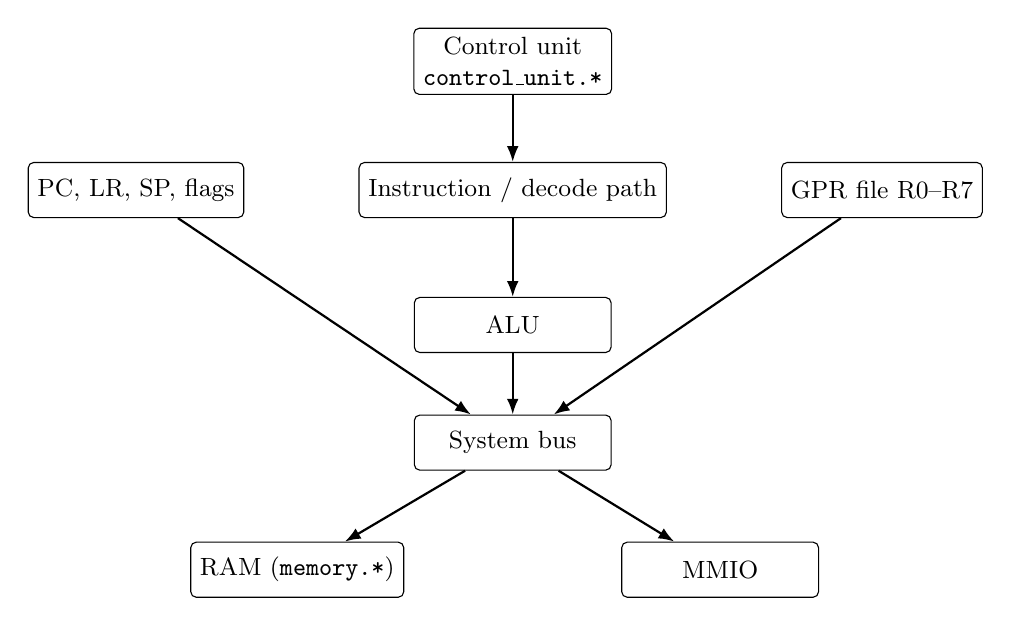
\begin{tikzpicture}[
    font=\small,
    box/.style={draw,rounded corners=2pt,minimum width=2.5cm,minimum height=0.7cm,align=center},
    arr/.style={-{Latex[length=2mm]},thick}
  ]
    \node[box] (cu) {Control unit\\\texttt{control\_unit.*}};
    \node[box,below=0.85cm of cu] (ir) {Instruction / decode path};
    \node[box,left=1.45cm of ir] (pc) {PC, LR, SP, flags};
    \node[box,right=1.45cm of ir] (gpr) {GPR file R0--R7};
    \node[box,below=1.0cm of ir] (alu) {ALU};
    \node[box,below=0.78cm of alu] (bus) {System bus};
    \node[box,below left=0.9cm and 0.12cm of bus] (ram) {RAM (\texttt{memory.*})};
    \node[box,below right=0.9cm and 0.12cm of bus] (mmio) {MMIO};
    \draw[arr] (cu) -- (ir);
    \draw[arr] (ir) -- (alu);
    \draw[arr] (pc) -- (bus);
    \draw[arr] (gpr) -- (bus);
    \draw[arr] (alu) -- (bus);
    \draw[arr] (bus) -- (ram);
    \draw[arr] (bus) -- (mmio);
  \end{tikzpicture}
  \caption{SPARTAN-16 CPU block diagram (fetch/decode/execute; RAM vs.\ MMIO).}
  \label{fig:cpu}
\end{figure}

\section{CPU design summary}
The CPU follows a FETCH $\rightarrow$ DECODE $\rightarrow$ EXECUTE pipeline implemented in the control unit (\texttt{control\_unit.*} in the repository). The register file exposes eight general-purpose registers plus stack pointer, link register, program counter, flags, and state needed to mirror the fetched instruction. The system bus routes ordinary RAM traffic separately from memory-mapped device ports.

\section{Instruction Set Architecture (ISA)}
\subsection{Instruction format}
Instructions are \textbf{four bytes} (32 bits) wide, fixed width, stored \textbf{little-endian}. The ISA combines R-type and I-type patterns; see \texttt{docs/isa.md} for bit-level layouts.

\subsection{Instructions and encoding}
The implementation provides \textbf{35 opcodes} spanning ALU operations (arithmetic, logic, shifts), memory access, branches, and stack operations. \texttt{docs/isa.md} is the authoritative opcode and encoding reference.

\subsection{Addressing modes}
Register operands, immediates where supported, PC-relative branches, and memory operands through load/store to calculated addresses are all documented in \texttt{docs/isa.md}.

\subsection{Flag semantics}
Condition codes \texttt{Z}, \texttt{N}, \texttt{C}, and \texttt{V} are updated after arithmetic ALU operations and are observable in \texttt{--trace} output.

\subsection{Memory map}
Physical memory is a 64\,KB byte array. Memory-mapped I/O occupies \texttt{0xF000}--\texttt{0xFFFF} (console, numeric print, timer, stdin per \texttt{README.md}). The active stack grows downward from \texttt{0xEFFE}. Executable binaries use an eight-byte header: bytes \texttt{0--3} are the magic ASCII sequence \texttt{SP16}; bytes \texttt{4--5} are the 16-bit little-endian load address; bytes \texttt{6--7} are the 16-bit little-endian payload length; program bytes follow immediately (see \texttt{emulator.cpp::load}).

\section{Emulator implementation}
\subsection{Registers}
The CPU state object (\texttt{cpu.*}) holds general-purpose registers, stack pointer, link register, program counter, flags, and auxiliary state required by the control unit.

\subsection{Arithmetic Logic Unit (ALU)}
\texttt{alu.*} implements arithmetic, logic, and shift operations and computes flag updates consistent with the ISA.

\subsection{Control unit}
\texttt{control\_unit.*} implements the FETCH $\rightarrow$ DECODE $\rightarrow$ EXECUTE loop, optionally emitting a structured trace when \texttt{--trace} is enabled.

\subsection{Bus}
\texttt{bus.*} demultiplexes reads and writes to RAM versus MMIO decode ranges.

\subsection{Memory}
\texttt{memory.*} backs the 64\,KB array; the loader copies post-header bytes into RAM starting at the header's load address and resets the CPU so the program counter matches that entry point.

\subsection{Memory-mapped I/O}
Demo programs interact with devices by issuing loads/stores to MMIO addresses documented in \texttt{docs/isa.md} and summarized in \texttt{README.md}.

\subsection{Load, run, and memory dump}
\texttt{./cpu run} executes a previously assembled \texttt{.bin} file. \texttt{./cpu exec} assembles and runs in one step. Execution runs until a halt condition; \texttt{--dump} prints a hex/ASCII view of the first 256 bytes of RAM after the run, matching the published demo script behavior.

\section{Assembler}
\subsection{Code production}
The two-pass assembler (\texttt{assembler.*}) emits the eight-byte binary header described above followed by raw program bytes consumable by the emulator loader.

\subsection{Labels and numeric literals}
Labels are resolved across both passes. Directives supported in-tree include \texttt{.org}, \texttt{.string}, \texttt{.word}, \texttt{.byte}, and \texttt{.align}, in addition to opcode mnemonics (see \texttt{docs/isa.md} for syntax details).

\section{Programs}
\subsection{Hello, World}
\texttt{programs/hello.asm} prints \texttt{Hello, World!} using MMIO character output. Run with \texttt{./cpu exec programs/hello.asm}; use \texttt{--trace} to capture every fetch/decode/execute cycle for documentation.

\subsection{Fibonacci sequence}
\texttt{programs/fibonacci.asm} prints the first ten Fibonacci numbers. The algorithm keeps a sliding window in registers \texttt{R0} and \texttt{R1}, uses \texttt{ADD} to advance the sequence, and prints via MMIO store operations. Compare register motion against the disassembly in \texttt{--trace} output when producing the required video.

\subsection{Timer example (Fetch / Compute / Store)}
\texttt{programs/timer.asm} counts from 1 to 10 and then prints the total CPU cycles consumed by the loop, highlighting repeated \textbf{fetch} (instruction retrieval), \textbf{compute} (ALU/control work for the counter), and \textbf{store} (MMIO updates) phases. Run with \texttt{./cpu exec programs/timer.asm} and optionally add \texttt{--trace} to show each instruction's contribution to the cycle budget.

\end{document}
